\clearpage
\section{Additional Details on CVAE Experiments}\label{app:detail}


\paragraph{Data preprocessing.}
We use MNIST ($28\times 28$ grayscale) and normalize pixel intensities to $[0,1]$. 
Class labels are represented as one-hot vectors $y\in\{0,1\}^{K}$ ($K{=}10$). 

\paragraph{Experiment Details.} 
We use a convolutional CVAE model consisting of an Encoder with two convolutional layers 
(1$\to$32 and 32$\to$64 channels, $4\times4$ kernels, stride 2, with GELU activations), 
followed by a linear projection that outputs the mean and log-variance of a $d_z=20$-dimensional 
Gaussian latent space. 
The Decoder mirrors this structure: a linear layer maps the latent code to a 
$64\times7\times7$ tensor, which is upsampled by two transposed convolutional layers 
(64$\to$32 and 32$\to$1 channels, $4\times4$ kernels, stride 2, with GELU activations) 
to reconstruct $28\times28$ images. 
We train the CVAE with the standard objective, i.e., binary cross-entropy reconstruction loss 
plus KL divergence regularization.


\paragraph{Discriminator for filtering.} 
We additionally train a discriminator $D$ to distinguish real from synthetic samples. 
$D$ is implemented as a multi-layer perceptron: five fully connected layers with hidden sizes 
512, 256, 128, and 64, each followed by a LeakyReLU activation, 
and a final linear layer mapping to a single logit. 
The output is passed through a sigmoid to yield the probability of the input being real. 
The discriminator is trained with binary cross-entropy, labeling real MNIST digits as positive 
and CVAE-generated digits as negative. 

\paragraph{Synthetic generation and filtering.}
After each training round, we generate conditioned samples by drawing 
$z \sim \mathcal{N}(0,I)$, choosing labels $y$ (uniform over classes unless specified), 
and decoding $\tilde{x} = g_{\theta}(z,y)$. 
To control sample quality, we score each $(\tilde{x},y)$ with the discriminator $D(\tilde{x},y)$. 
For each class, we retain only the top $10\%$ of generated samples with the highest discriminator 
scores. These filtered synthetic samples are then combined with the real dataset to form the 
training data for the next round. 


\paragraph{Supplementary Results on ELBO}
\textcolor{black}{
We also evaluate generative performance using the test negative ELBO, a standard likelihood-based loss metric for VAEs. 
To prevent overfitting the discriminator (i.e., the verifier) and ensure stability during the retraining cycles, we incorporate standard regularization techniques, specifically applying a dropout rate of 0.1 and label smoothing with a parameter of 0.05 when training the discriminator.
To investigate the effect of synthetic data size $n_k$, we employ three linearly increasing sample size schedules.
Starting with an initial CVAE trained on only 500 samples, we scale up the retraining size by adding 5K, 30K, or 50K synthetic samples per iteration, respectively.
The models are retrained for 50 iterations until the test negative ELBO stabilizes.}

Figure~\ref{fig:iter_recon_loss} reports the test negative ELBO over these 50 rounds.
Consistent with our bias--variance analysis, we observe a clear improvement (a decrease in loss) in the early stages (up to roughly iterations 10--15).
Furthermore, the trajectories reveal a critical dynamic: while larger synthetic size schedules significantly accelerate this early convergence, all three schedules ultimately plateau and converge to a similar negative ELBO value by iteration 50. 
This observation validates our theoretical framework: drawing more synthetic samples expedites the initial variance reduction phase, but the asymptotic performance limit is dictated by the verifier, not the volume of synthetic data.
After the initial variance-reduction gains, the negative ELBO eventually reverses its trend and increases (deteriorates) as the model inevitably converges toward the verifier's knowledge center.

As discussed in the main text regarding our verifier's limitations, this knowledge center is demonstrably biased.
For reference, across all three size schedules, the final retrained CVAEs at iteration 50 converge to a test negative ELBO of approximately 111. In contrast, a baseline CVAE trained on the entire 60K real image dataset attains a test negative ELBO of 92.12 (lower is better).
Because our verifier emphasizes perceptual quality over likelihood-based reconstruction, the negative ELBO proves harder to improve than FID. 
As a result, even as the negative ELBO stagnates or worsens in later iterations, our retrained models continue to improve FID, achieving sharper, cleaner digits.
We believe that deploying stronger verifiers with, e.g., diversity preservation capabilities could enable iterative retraining to further improve the negative ELBO.



\begin{figure}[H]
    \centering
    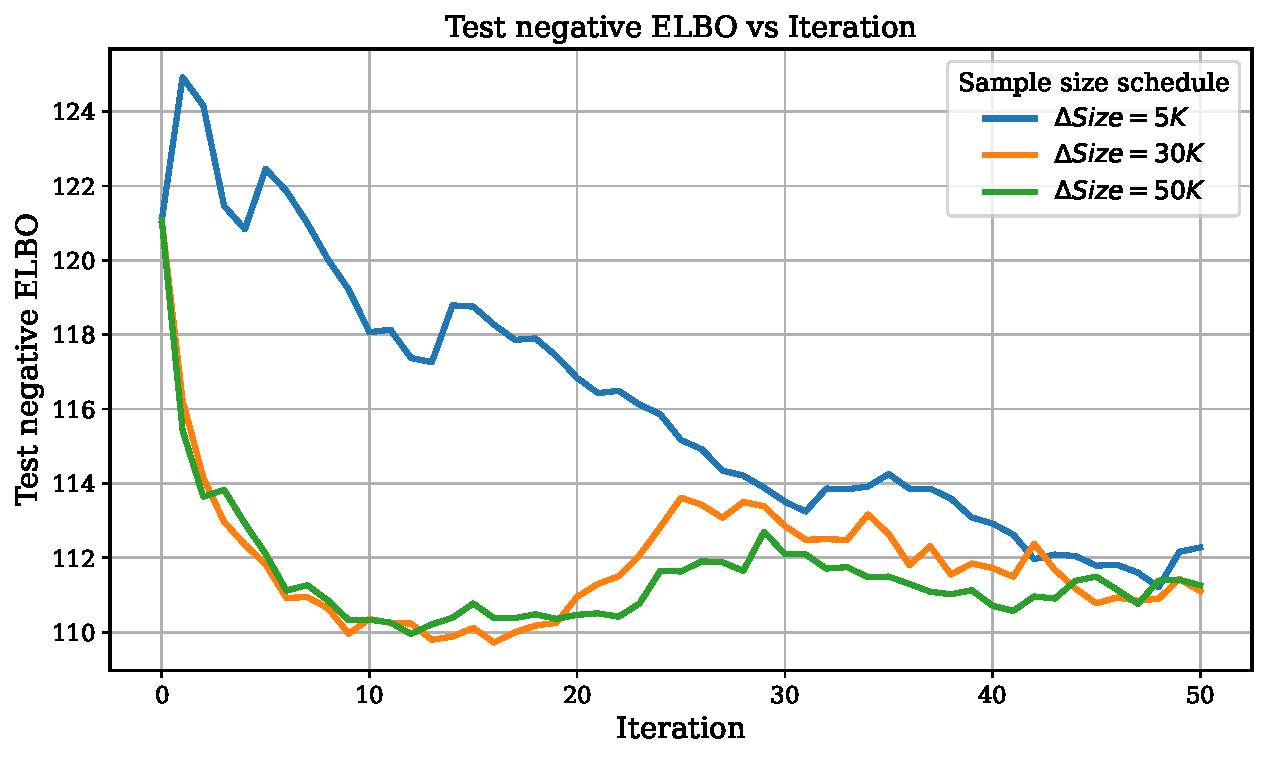
\includegraphics[width=0.6\textwidth]{./plot/fig_ELBO_labelsmoothed.pdf}
    \caption{Test negative ELBO across retraining iterations.}
    \label{fig:iter_recon_loss}
\end{figure}

\section{Additional Experimental Results}\label{app:addexp}

\subsection{Random Synthetic Data in Linear Regression}\label{sec:random_synthetic_data}


In the main text, the synthetic covariates were aligned with a fixed orthonormal basis to
simplify analysis and make the retraining dynamics easier to interpret. To show that the
observed behavior is not tied to this structured design, we repeat the same iterative
retraining experiment using fully random synthetic covariates sampled i.i.d.\ from a
standard Gaussian distribution.

Figure~\ref{fig:linear_random} presents the results, corresponding directly to the lower two
panels in Figure~\ref{fig:linear_combined} of the main text, but under the random-design
setting. The qualitative behavior remains the same: with a well-specified verifier,
retraining contracts toward the verifier's knowledge center and avoids collapse, whereas
unfiltered retraining diverges. This confirms that the verifier-induced stability and
improvement patterns hold beyond the orthonormal-design assumption.

\begin{figure}[H]
    \centering
    \begin{subfigure}[b]{0.495\textwidth}
        \centering
        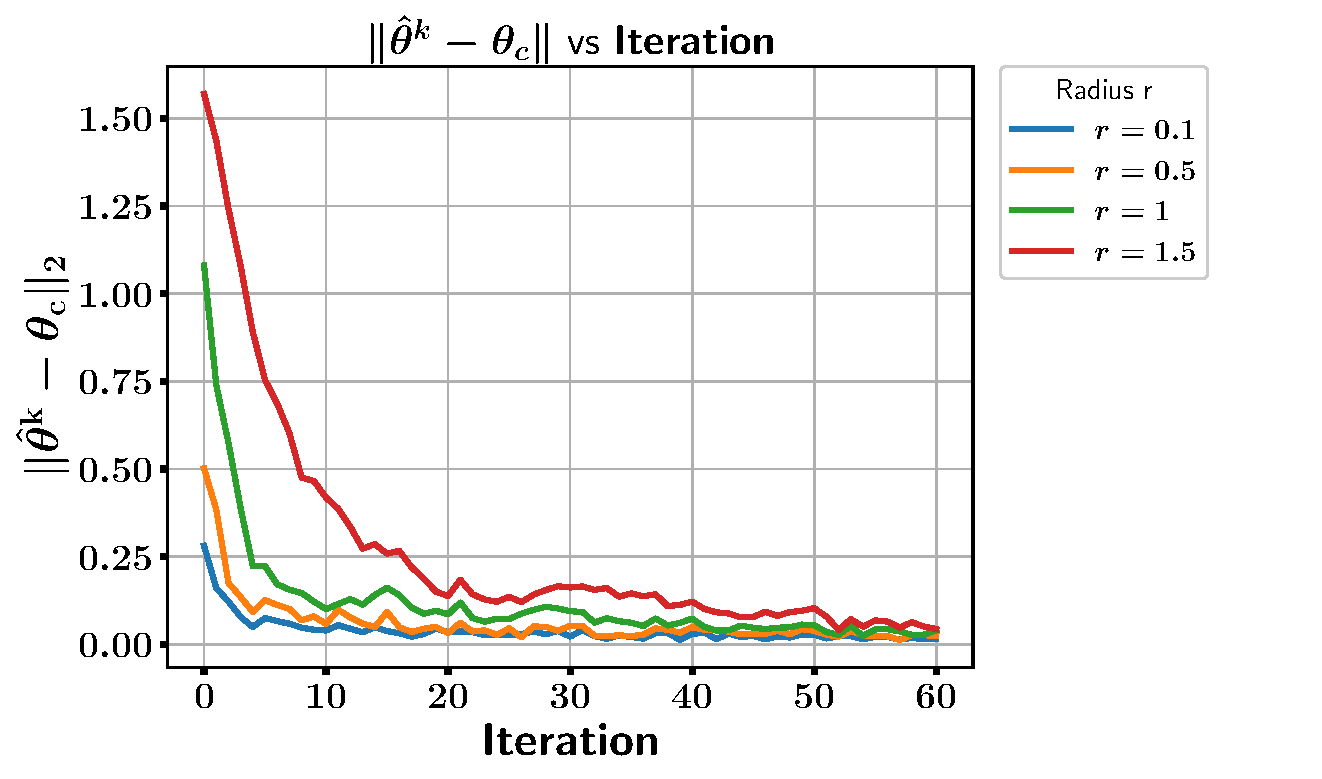
\includegraphics[width=\linewidth]{./plot/linear1_random_2_random_direction.pdf}
        \caption{Verifier with bias (random design)}
    \end{subfigure}
    \hfill
    \begin{subfigure}[b]{0.495\textwidth}
        \centering
        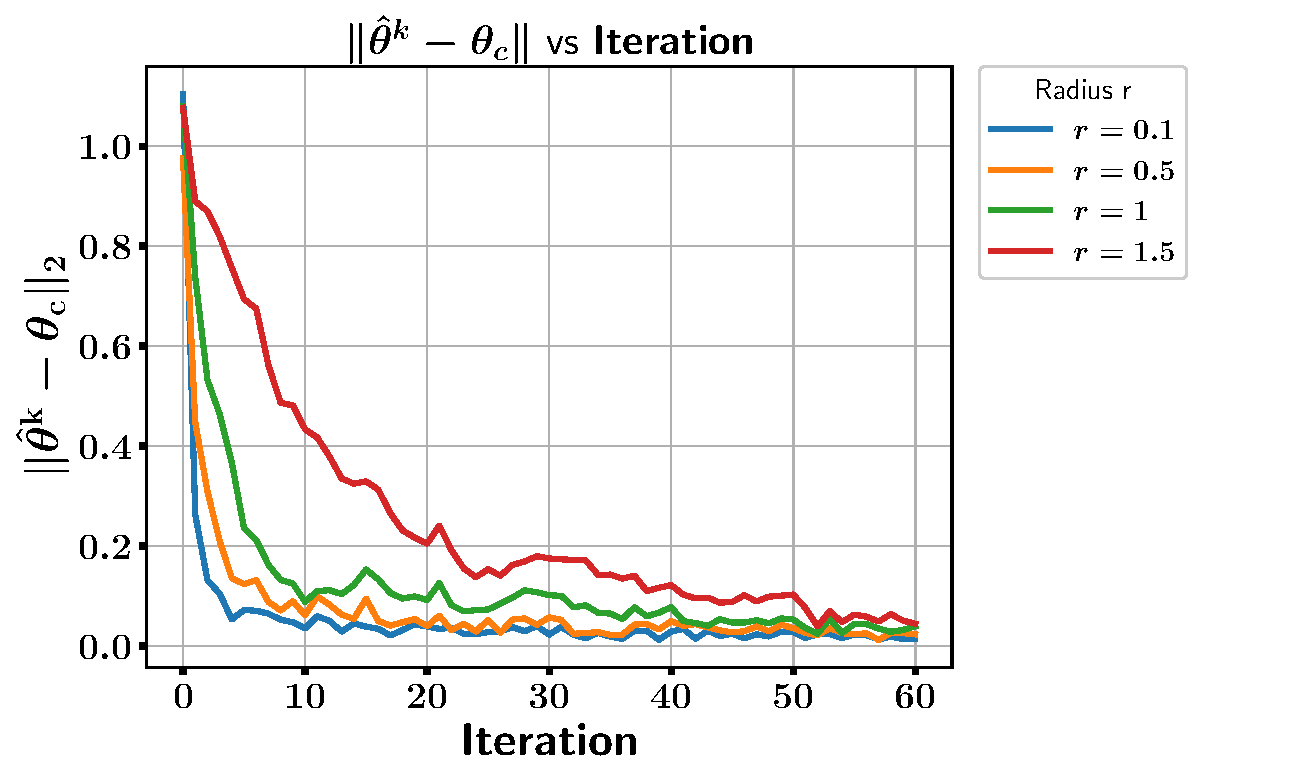
\includegraphics[width=\linewidth]{./plot/linear1_random_2.pdf}
        \caption{Verifier without bias (random design)}
    \end{subfigure}
    \caption{{Iterative synthetic retraining under random synthetic covariates, 
    corresponding to the structured-design results in Figure~\ref{fig:linear_combined}.}}
    \label{fig:linear_random}
\end{figure}
\subsection{Different Verifier Shapes}\label{sec:verifier_shape}

We further analyze how different geometric choices of the verifier region affect the
acceptance rule and the resulting retraining dynamics.
For any region $\mathcal{R}_\theta$ around a center $\theta_c$, a synthetic point
$(x,y)$ is accepted whenever there exists a parameter perturbation $\Delta$ in the
region that can explain $y$, i.e.
\[
   y = x^\top (\theta_c + \Delta) + \xi, \qquad \Delta \in \mathcal{R}_\theta.
\]
This leads to the general acceptance requirement
\[
   |y - x^\top \theta_c|
   \le \sup_{\Delta \in \mathcal{R}_\theta} |x^\top \Delta| + \sigma_c.
\]
Different verifier shapes correspond to different support functions 
$\sup_{\Delta \in \mathcal{R}_\theta} |x^\top \Delta|$.

\paragraph{(1) Ellipsoidal verifier.}
Consider the anisotropic ellipsoid
\[
    \mathcal{R}_\theta = \bigl\{
        \theta : (\theta - \theta_c)^\top A(\theta - \theta_c) \le r^2
    \bigr\}, \qquad A \succ 0.
\]
Let $\Delta = \theta - \theta_c$.  
Changing variables $\Delta = A^{-1/2}u$ with $\|u\|_2 \le r$ yields
\[
    \sup_{\Delta^\top A \Delta \le r^2} |x^\top \Delta|
    = r\|A^{-1/2}x\|_2
    = r\sqrt{x^\top A^{-1}x}.
\]
Thus the acceptance condition becomes
\[
    |y - x^\top \theta_c|
    \le r\sqrt{x^\top A^{-1}x} + \sigma_c.
\]

\paragraph{(2) Polyhedral $\ell_1$ verifier.}
For the $\ell_1$ knowledge region
\[
    \mathcal{R}_\theta = \{\|\theta - \theta_c\|_1 \le r\},
\]
the perturbation satisfies $\|\Delta\|_1 \le r$.  
Using Hölder duality,
\[
    \sup_{\|\Delta\|_1 \le r} |x^\top \Delta|
    = r\|x\|_\infty.
\]
The corresponding acceptance rule is
\[
    |y - x^\top \theta_c|
    \le r\|x\|_\infty + \sigma_c.
\]

Although ellipsoidal and $\ell_1$ (polyhedral) regions induce different forms of 
acceptance sets, both yield the same qualitative retraining behavior:
\emph{$\hat{\theta}^{(k)}$ consistently move toward the verifier center $\theta_c$}. The empirical trajectories under both shapes are shown in Figure~\ref{fig:verifier-shapes}.

\begin{figure}[H]
    \centering

    % ------- Ellipsoidal verifier (first) -------
    \begin{subfigure}[b]{0.495\textwidth}
        \centering
        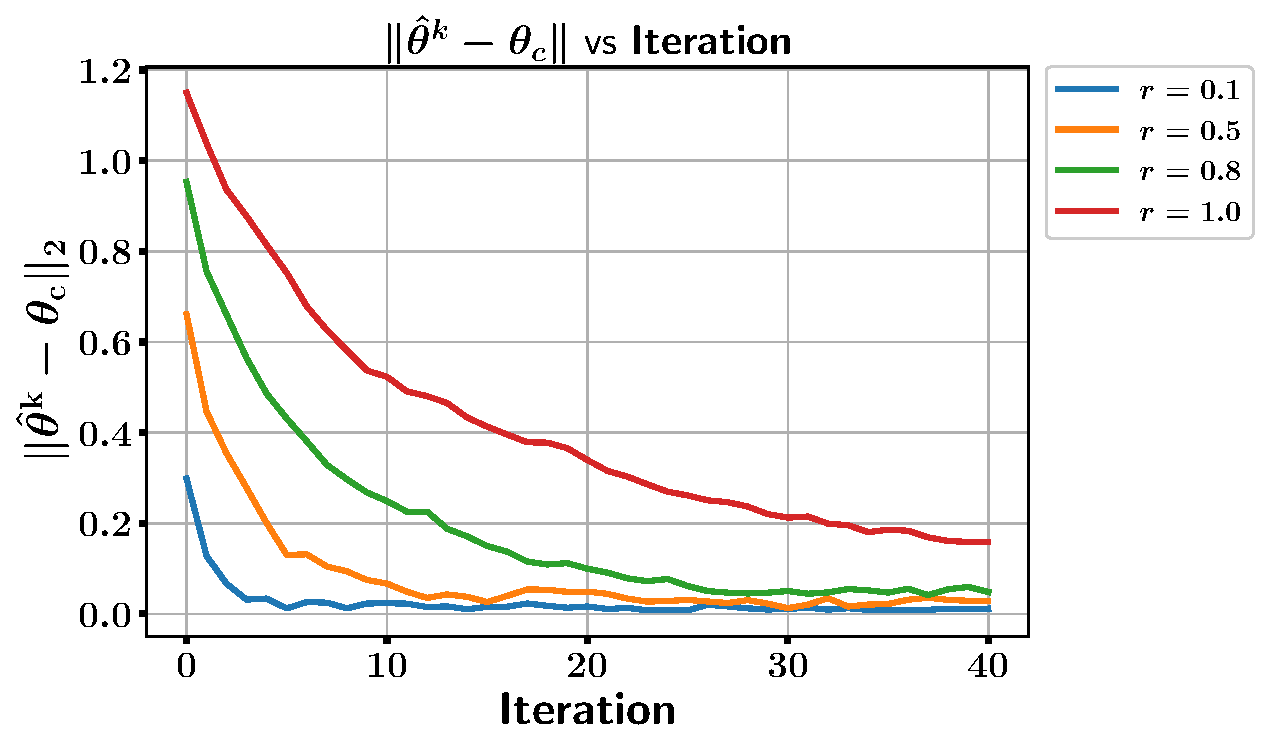
\includegraphics[width=\linewidth]{./plot/ellipsoid.pdf}
        \caption{Ellipsoidal verifier}
    \end{subfigure}
    \hfill
    % ------- L1 verifier (second) -------
    \begin{subfigure}[b]{0.495\textwidth}
        \centering
        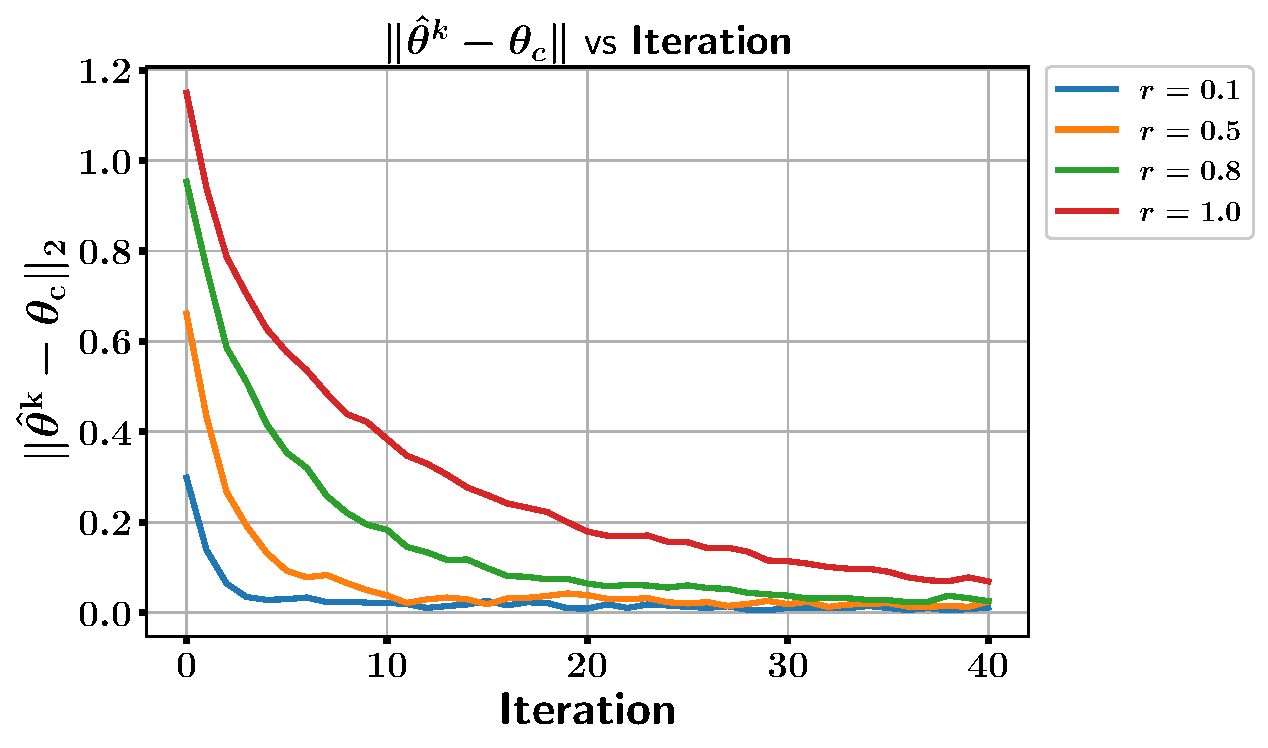
\includegraphics[width=\linewidth]{./plot/l1.pdf}
        \caption{Polyhedral $\ell_1$ verifier}
    \end{subfigure}

    \caption{Retraining trajectories under two different verifier shapes.  
    In both cases, $\hat{\theta}^{(k)}$ empirically converges toward the 
    verifier center $\theta_c$.}
    \label{fig:verifier-shapes}
\end{figure}


\subsection{MNIST-Specific FID Evaluation}
\label{sec:mnist-fid}
The standard Fréchet Inception Distance (FID) is widely used in generative modeling, including on MNIST, following prior work such as \citet{daidiagnosing,leontev2020quality,chan2024evaluating}.  Nonetheless, we agree that Inception embeddings are not tailored to handwritten digits and may not fully capture perceptual similarity on MNIST.

To address this point, we introduce a \textbf{MNIST-specific FID} variant.  
We train a lightweight convolutional network directly on MNIST classification, and compute FID using the penultimate-layer activations as the embedding space.  
This produces a domain-appropriate FID measure while preserving the same statistical structure as the original metric. These results confirm that our conclusions are robust to the choice of embedding and do not depend on the use of vanilla FID.

\vspace{0.5em}
\noindent\textbf{Results.}
Figures~\ref{fig:mnist-fid-v2-full} and \ref{fig:mnist-fid-v2-zoom} report the new FID scores under our retraining framework for all verifier sizes.  
Consistent with the standard FID curves in the main paper.
\begin{figure}[H]
    \centering
    \begin{subfigure}[t]{0.495\textwidth}
        \centering
        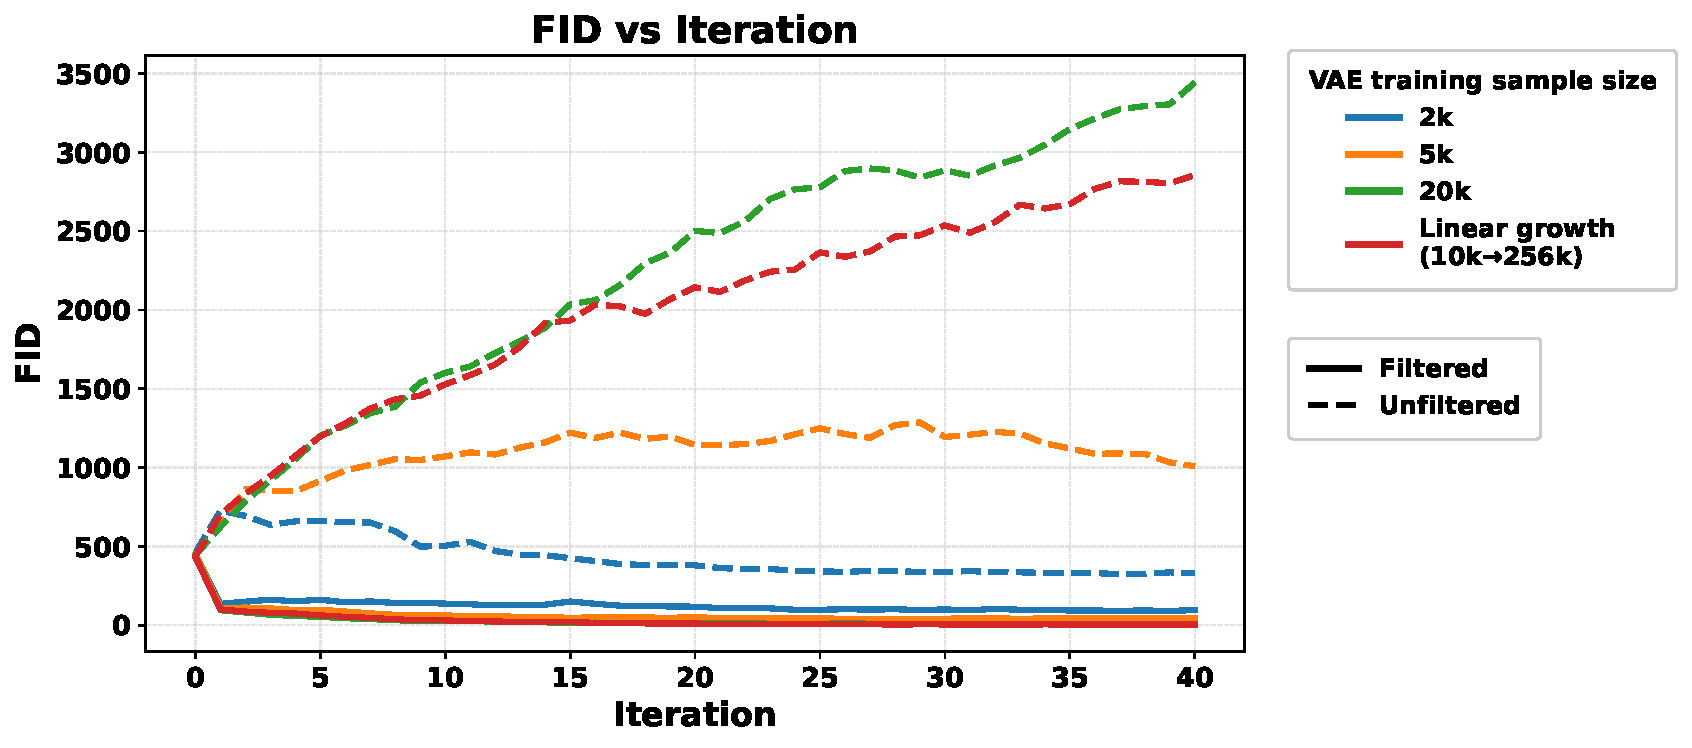
\includegraphics[width=\linewidth]{./plot/new_fid_v2_fixed.pdf}
        \caption{\textbf{MNIST-specific FID over retraining iterations.}}
        \label{fig:mnist-fid-v2-full}
    \end{subfigure}
    \hfill
    \begin{subfigure}[t]{0.495\textwidth}
        \centering
        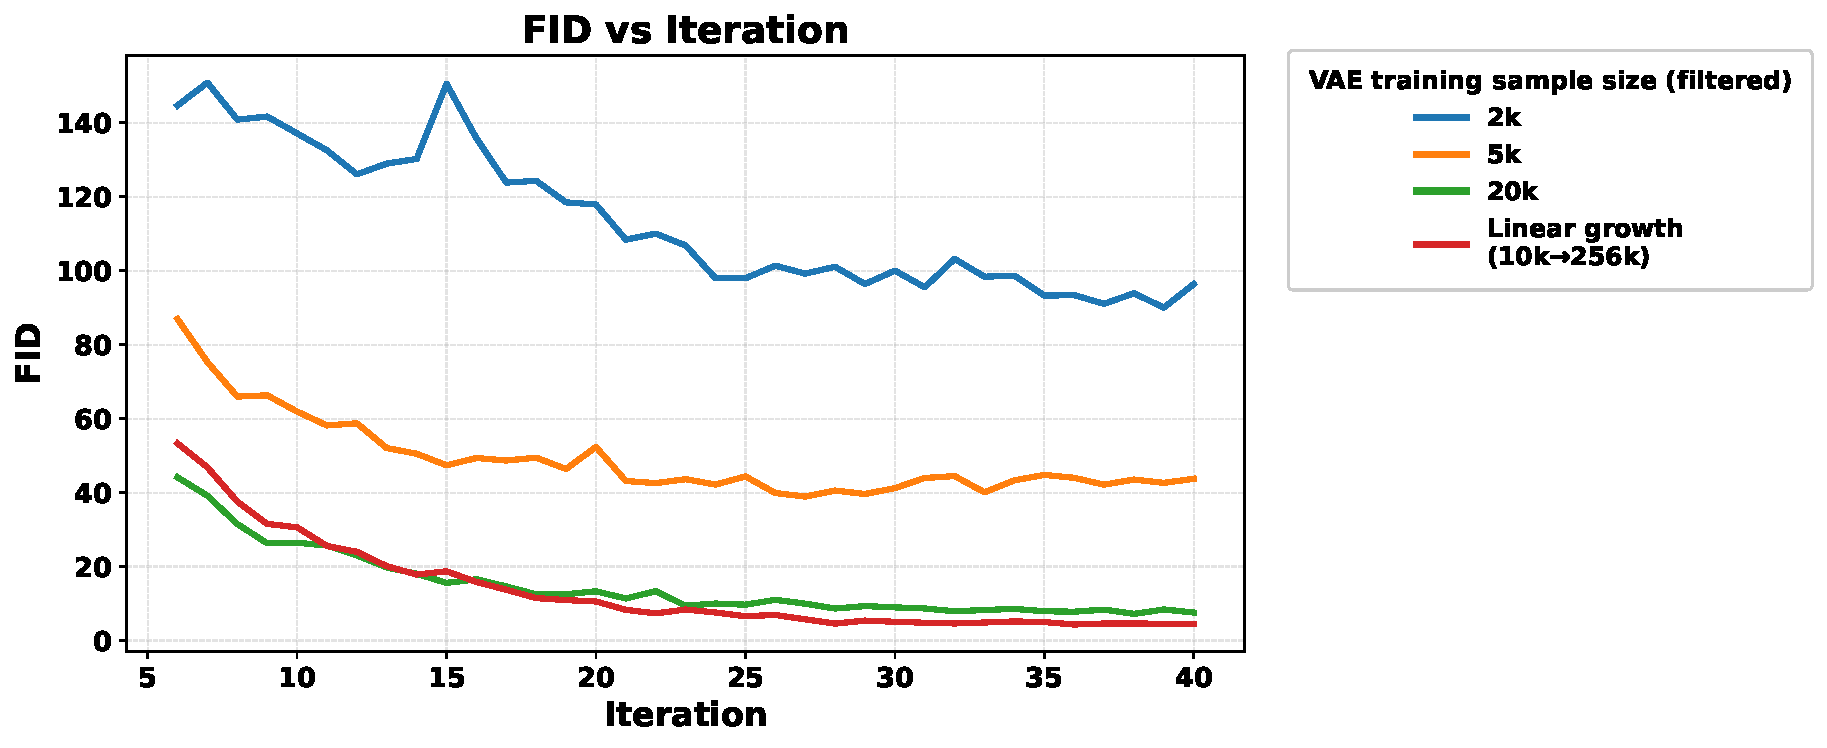
\includegraphics[width=\linewidth]{./plot/new_fid_v2_filtered_after5.pdf}
        \caption{\textbf{Zoom-in view for filtered runs.}}
        \label{fig:mnist-fid-v2-zoom}
    \end{subfigure}
    \caption{\textbf{MNIST-specific FID using our MNIST-trained feature embedding.}  
    Both results confirm that our conclusions remain unchanged when replacing standard FID with a domain-specific metric.}
    \label{fig:mnist-fid-v2-both}
\end{figure}

\subsection{Different Initial Sample Sizes}\label{sec:initial_sample_size}

We assess the robustness of verifier-guided retraining by varying the number of real
MNIST images used to train the initial CVAE ($1k, 2k, 3k, 4k, 60k$). For small and
medium initial sample sizes, verifier filtering yields clear early FID improvements and then stabilizes performance, whereas unfiltered retraining quickly degrades. When the
generator is initialized on all 60k real images, verifier filtering no longer improves FID over the initial model, but it still effectively prevents the severe collapse observed under
unfiltered retraining.

We perform our main experiments in a low–real-data regime (e.g., with 500 initial images), where the verifier, having been trained on a much larger subset of MNIST, holds strictly more external knowledge than the generator. According to our theory, this is exactly the regime in which verifier-guided retraining should provide true improvement rather than simple stabilization, because the verifier contributes additional information. In contrast, when the generator is initialized on the full 60k training images,
the verifier would need access to an even stronger source of external information to
achieve improvement; otherwise it can only prevent collapse. For this reason, the small
initial sample size serves as the most informative regime for highlighting the verifier’s
knowledge-injection effect and demonstrating the improvement phenomena predicted
by our theoretical framework.

\begin{figure}[H]
    \centering
    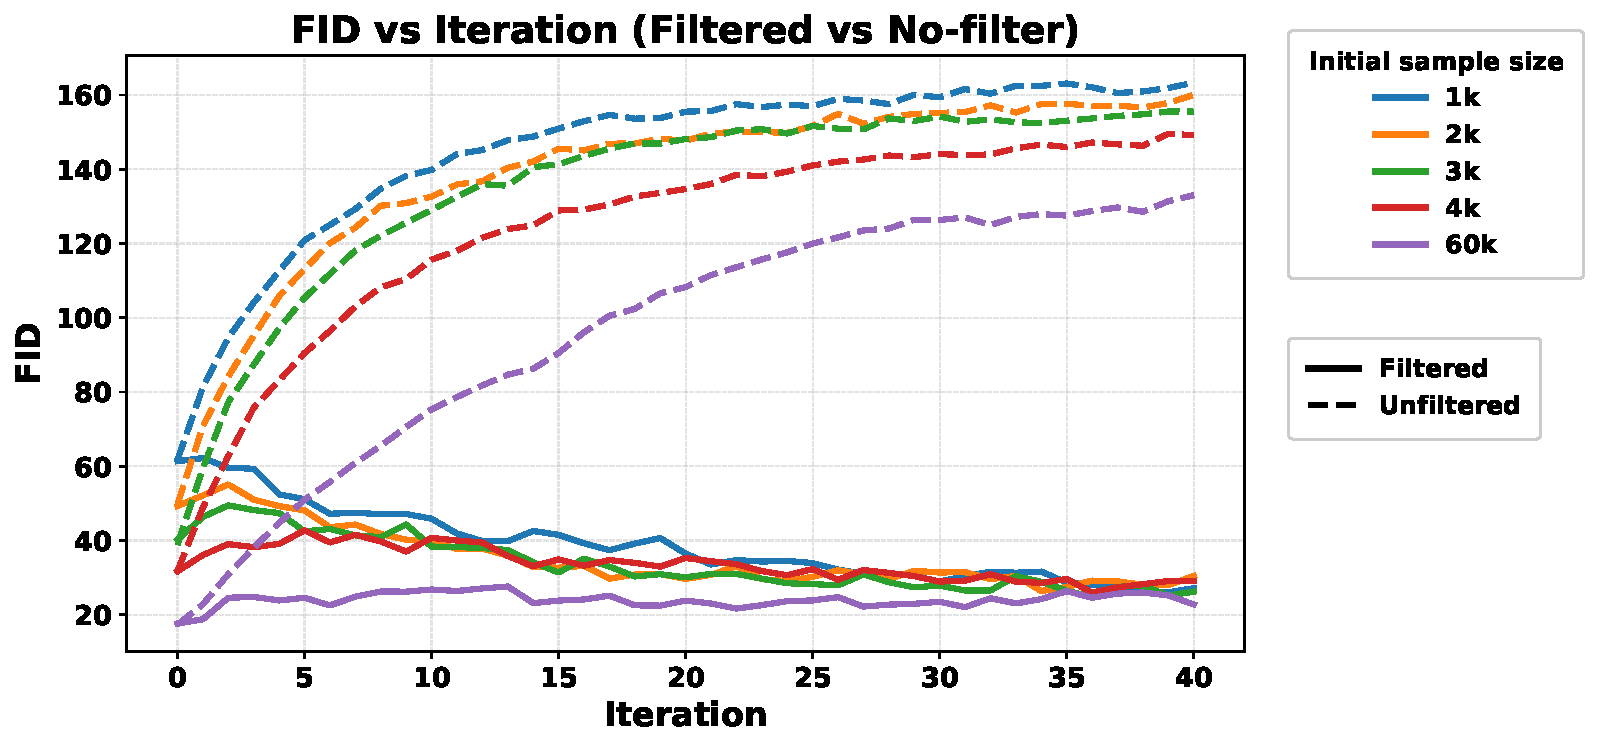
\includegraphics[width=0.55\linewidth]{./plot/fid_filtered_vs_nofilter.pdf}
    \caption{FID across retraining iterations under different initial sample sizes, 
    comparing verifier-filtered and unfiltered synthetic retraining.}
    \label{fig:placeholder}
\end{figure}